\subsubsection{Presentacion de estudiente para su curso}

{\textbf {Resumen:}}
Un alumno de enseñanza media tiene que hacer una presentación sobre un tema histórico local, el recuerda que hay informacion de esto en el museo pero no puede ir por cuarentena (COVID), a su vez recuerda que en la aplicación “museo en casa” tiene esa pieza en su colección, días después el estudiante presenta sin problemas ya que pudo obtener la información necesaria para esta desde la información entregada por la aplicación.

{\textbf {Actores:}}
Estudiante.

{\textbf {Propósito:}}
Mostrar usos prácticos de la aplicación que no tengan una relación directa con su parte lúdica.

{\textbf {Referencias cruzadas:}}
R1.1, R1.2, R2.7,R2.8, R5.3, R6.1, R6.5

\paragraph{Caso de Uso Esencial}

\begin{longtable}{|p{5cm}|p{8cm}|}
\hline 
Acción actores & Respuesta del sistema \\ 
\hline 
XXXX & XXXX \\ 
\hline 
\end{longtable}

\paragraph{Diagrama de Caso de Uso}

\begin{figure}[H]
\centerline{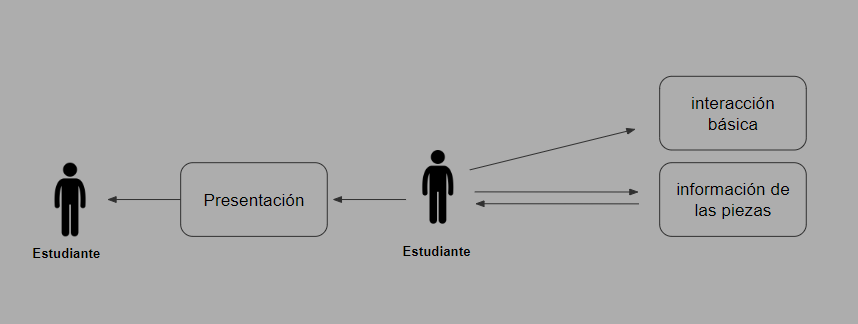
\includegraphics[width=15cm]{imgs/CasoUso_4.PNG}}
\caption{Caso-1}
\label{fig}
\end{figure}

\paragraph{Modelo Conceptual}

%\begin{figure}[H]
%\centerline{\includegraphics[width=15cm]{imgs/CasoUso_1_3.PNG}}
%\caption{Caso-1}
%\label{fig}
%\end{figure}

\paragraph{Diagrama de Secuencia o Colaboración}

\begin{figure}[H]
\centerline{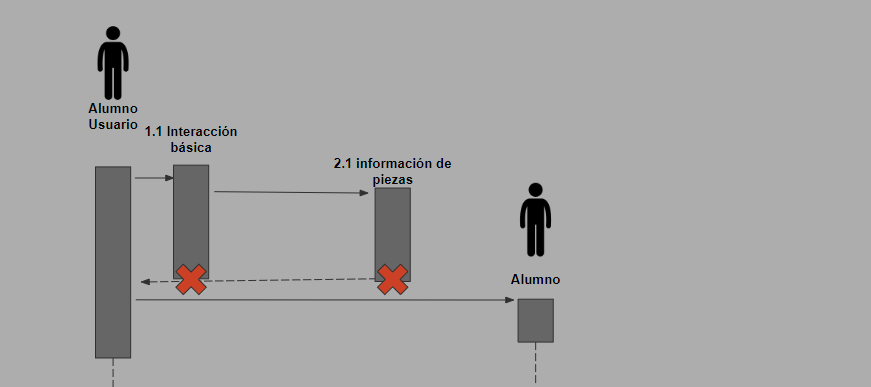
\includegraphics[width=15cm]{imgs/CasoUso_4_2.PNG}}
\caption{Caso-1}
\label{fig}
\end{figure}

\paragraph{Priorización}
{\textbf {Tipo:}}
Deseable.